\documentclass[11pt,letterpaper, leqno]{article}
\usepackage{latexsym}
\usepackage{amsmath}
\usepackage{amssymb}
\usepackage{amsthm}
\usepackage{tikz}

\topmargin -0.25in
\textheight 8.5in
\oddsidemargin 0.0in
\textwidth 6.5in

\RequirePackage{amsthm,amsmath,amsfonts,amssymb}
%\RequirePackage[numbers]{natbib}
\RequirePackage[authoryear]{natbib}%% uncomment this for author-year citations
\RequirePackage[colorlinks,citecolor=blue,urlcolor=blue]{hyperref}%% uncomment this for coloring bibliography citations and linked URLs
\RequirePackage{graphicx}%% uncomment this for including figures

\usepackage{natbib}
\usepackage{authblk}
\usepackage[english]{babel}
\bibliographystyle{abbrvnat}
\setcitestyle{authoryear,open={(},close={)}}

% For the algorithm table
\usepackage{algorithm,algcompatible,amsmath}
\DeclareMathOperator*{\argmax}{\arg\!\max}
\DeclareMathOperator*{\argmin}{\arg\!\min}
% https://tex.stackexchange.com/q/83169/5764
\algnewcommand\INPUT{\item[\textbf{Input:}]}%
\algnewcommand\OUTPUT{\item[\textbf{Output:}]}%
%

\newtheorem{theorem}{Theorem}
\newtheorem{acknowledgement}[theorem]{Acknowledgement}
%\newtheorem{algorithm}[theorem]{Algorithm}
\newtheorem{axiom}[theorem]{Axiom}
\newtheorem{problem}[theorem]{Problem}
\newtheorem{remark}{Remark}
\newtheorem{claim}[theorem]{Claim}
\newtheorem{conclusion}[theorem]{Conclusion}
\newtheorem{condition}[theorem]{Condition}
\newtheorem{conjecture}[theorem]{Conjecture}
\newtheorem{corollary}{Corollary}
\newtheorem{criterion}[theorem]{Criterion}
\newtheorem{definition}{Definition}
\newtheorem{example}{Example}
\newtheorem{exercise}[theorem]{Exercise}
\newtheorem{lemma}{Lemma}
\newtheorem{proposition}{Proposition}
\newtheorem{thm}{Theorem}[section]
\newtheorem{lem}{Lemma}[section]
\newtheorem{prop}{Proposition}[section]
\newtheorem{defn}{Definition}[section]
\newtheorem{ex}{Example}[section]
\newtheorem{cor}{Corollary}[section]
\newtheorem{rem}{Remark}[section]
\newtheorem{rems}{Remarks}[section]
\numberwithin{equation}{section} 
\numberwithin{theorem}{section}
\numberwithin{lemma}{section} 
\numberwithin{corollary}{section}
\numberwithin{definition}{section}
\numberwithin{proposition}{section} 
\numberwithin{remark}{section}
\numberwithin{example}{section}
\newtheorem{assumption}{Assumption}
\DeclareMathOperator\supp{supp}

%\newcommand{\ex}{{\bf\sf E}}            %% expectation
\newcommand{\bfp}{{\bf P}}
\newcommand{\bfr}{{\bf R}}
\newcommand{\Var}{{\rm Var}}            %% 
\newcommand{\Cov}{{\rm Cov}}            %% 
\newcommand{\calc}{{\cal C}}            %%
\newcommand{\cald}{{\cal D}} 
\newcommand{\calf}{{\cal F}}            %%
\newcommand{\call}{{\cal L}}            
\newcommand{\al}{\alpha}                %%
\newcommand{\bt}{\beta}                %%
\newcommand{\ga}{\gamma}                %% abbreviated
\newcommand{\dt}{\delta}                %% greek letters
\newcommand{\la}{\lambda}               %%
\newcommand{\ep}{\epsilon}              %%
\newcommand{\sig}{\sigma}               %%
\newcommand{\tri}{\triangle}
\newcommand{\om}{\omega}                %%
\newcommand{\ra}{\rightarrow}           %%
\newcommand{\lra}{\longrightarrow}
\newcommand{\Ra}{\Rightarrow}           %% arrows
\newcommand{\subs}{\subseteq}           %% subset or equal to
\newcommand{\eqdef}{\stackrel{\triangle}{=}}
\newcommand{\hY}{\hat{Y}}
\newcommand{\hp}{\hat{p}}
\newcommand{\hX}{\hat{X}}
\newcommand{\hy}{\hat{y}}
\newcommand{\hQ}{\hat{Q}}
\newcommand{\Zh}{\hat{Z}}
\newcommand{\hla}{\hat{\lambda}}
\newcommand{\starti}{\parindent0pt\it}  %% start an italic line
\newcommand{\startb}{\parindent0pt\bf}  %% start a boldface line
\newcommand{\tril}{\triangle^-}
\newcommand{\trir}{\triangle^+}
\newcommand{\trilr}{\triangle^{\pm}}
\newcommand{\realR}{{{\rm I}\;\!\!\!{\rm R}}}
\newcommand{\probP}{{{\rm I}\;\!\!\!{\rm P}}}
\newcommand{\filtF}{{{\rm I}\;\!\!\!{\rm F}}}
\newcommand{\expeE}{{{\rm I}\;\!\!\!{\rm E}}}
\newcommand{\noin}{{\noindent}}
\newcommand{\doty}{{\dot{y}}}
\newcommand{\doth}{{\dot{h}}}
\newcommand{\dotx}{{\dot{x}}}
\newcommand{\dotu}{{\dot{u}}}
\newcommand{\dotf}{{\dot{f}}}
\newcommand{\dotg}{{\dot{g}}}
\newcommand{\ddoty}{{\ddot{y}}}
\newcommand{\ddoth}{{\ddot{h}}}
\newcommand{\ddotx}{{\ddot{x}}}
\newcommand{\ddotf}{{\ddot{f}}}
%\newcommand{\Var}{{\mbox{Var}}}
%\newcommand{\Cov}{{\mbox{Cov}}}
\newcommand{\T}{\intercal}

\newcommand{\ans}[1]{\boxed{\text{#1}}}
\newcommand{\vecs}[1]{\langle #1\rangle}
\renewcommand{\hat}[1]{\widehat{#1}}
\newcommand{\F}[1]{\mathcal{F}(#1)}
\renewcommand{\P}{\mathbb{P}}
\newcommand{\R}{\mathbb{R}}
\newcommand{\E}{\mathbb{E}}
\newcommand{\Z}{\mathbb{Z}}
\newcommand{\ind}{\mathbbm{1}}
\renewcommand{\qed}{\quad \blacksquare}
\newcommand{\brak}[1]{\left\langle #1 \right\rangle}
\newcommand{\bra}[1]{\left\langle #1 \right\vert}
\newcommand{\ket}[1]{\left\vert #1 \right\rangle}
\newcommand{\bfP}{\mathbf{P}}
\newcommand{\mfX}{\mathfrak{X}}

\begin{document}
\begin{center}
{\bf \Large APMA1690: ~~Homework \# 6 ~~~(Due by 11pm on November 2)}
\end{center}
\[\]
\medskip

\section{Review}

I would suggest you go through the review section before going to the problem set.

\subsection{Notations}
\begin{itemize}
    \item $\mathbb{Z}$ = the collection of all integers.
    \item $\mathbb{Z}^d= \underbrace{\mathbb{Z} \times \mathbb{Z} \times \cdots \times \mathbb{Z}}_{\mbox{\href{https://en.wikipedia.org/wiki/Cartesian_product}{Cartesian product}, $d$ times}}$.
    \item For a Markov chain (MC) $\{X_n\}_{n=0}^\infty$, the subscript $n$ is conventionally referred to as ``time."
    \item Let $\boldsymbol{A}$ be a matrix. The \href{https://en.wikipedia.org/wiki/Transpose}{transpose} of $\boldsymbol{A}$ is denoted as $\boldsymbol{A}^\T$.
        \item Let $\boldsymbol{P}$ be an $S$-by-$S$ matrix. $\boldsymbol{P}^n=\underbrace{\boldsymbol{P}\boldsymbol{P}\cdots\boldsymbol{P}}_{\mbox{matrix multiplication, $n$ matrices}}$
    \item $(\boldsymbol{P}^n)_{ij}=$ the entry in the $i^{th}$ row and $j^{th}$ column of the matrix $\boldsymbol{P}^n$.
\end{itemize}


\subsection{Notation $\rho_{xy}$}

Let $\{X_n\}_{n=0}^\infty$ be a homogeneous Markov chain taking values in the discrete state space $\mathcal{X}$, which can be either finite or infinite. Recall that each $X_n$, for a fixed $n$, is a random variable, i.e., 
\begin{align*}
    X_n: \ \  & \Omega \rightarrow\mathcal{X}, \\
    & \omega \mapsto X_n(\omega).
\end{align*}
For the Markov chain and each element $y\in\mathcal{X}$, we define the following random variable
\begin{align*}
    T_y(\omega) &\overset{\operatorname{def}}{=}\min\left\{ n>0\, \,\vert\, X_n(\omega)=y\right\} \\
    &= \mbox{ the time at which the sequence $\{X_n(\omega)\}_{n=1}^\infty$ first visits }y.
\end{align*}
Here, we explicitly write down $\omega$ to emphasize that $T_y$ is a random variable. We denote the following probability, which will be used to define ``recurrence/transience" and ``irreducibility."
\begin{align*}
    \rho_{xy}&\overset{\operatorname{def}}{=}\mathbb{P}(T_y<\infty \,\vert \, X_0=x) \\
    & = \mbox{the conditional probability that MC will visit $y$ at least once, given that it starts from $x$.}
\end{align*}


\subsection{Transition Matrices}

Let $\{X_n\}_{n=0}^\infty$ be a homogeneous Markov chain whose state space is $\mathcal{X}=\{x_1,x_2,\ldots, x_S\}$ (where $S<\infty$) and having transition probability $p$. We define the following \textbf{transition matrix} of the Markov chain
\begin{align}\label{eq: transition matrix}
    \boldsymbol{P}=
    \begin{pmatrix}
    p(x_1, x_1) & p(x_1, x_2) & \cdots & p(x_1, x_S) \\
    p(x_2, x_1) & p(x_2, x_2) & \cdots & p(x_2, x_S) \\
    \vdots & \vdots & \ddots & \vdots \\
    p(x_S, x_1) & p(x_S, x_2) & \cdots & p(x_S, x_S)
    \end{pmatrix}.
\end{align}
It is straightforward that $\sum_{j=1}^S \boldsymbol{P}_{ij}=\sum_{j=1}^S p(x_i, x_j)=1$ for all $i\in\{1,2,\ldots,S\}$.

%\[\mathbb{P}( A \,\vert\, C) = \sum_{i=1}^n \mathbb{P}( A \,\vert\, C \cap B_i )\cdot \mathbb{P}( B_i \,\vert\, C) \]

\subsection{Irreducibility}

\begin{definition}
Let $\{X_n\}_{n=0}^\infty$ is a homogeneous Markov chain taking values in the discrete state space $\mathcal{X}$ and having transition probability $p$.
\begin{enumerate}
    \item The Markov chain $\{X_n\}_{n=0}^\infty$ or transition probability $p$ is said to be \textbf{recurrent} if all states of $\mathcal{X}$ are recurrent for this Markov chain.
    \item The Markov chain $\{X_n\}_{n=0}^\infty$ or transition probability $p$ is said to be \textbf{irreducible} if $\rho_{xy}>0$ for all $x,y\in\mathcal{X}$, i.e., we have a positive probability of transiting between any two states.
\end{enumerate}
\end{definition}

Because of the following theorem, the scenario where the state space $\mathcal{X}$ is finite is of importance in the Markov chain theory.
\begin{theorem}\label{thm: a finite state chain must have a recurrent state}
Let $\{X_n\}_{n=0}^\infty$ be a homogeneous Markov chain taking values in the state space $\mathcal{X}$. If $\mathcal{X}$ is finite, we have
\begin{enumerate}
    \item $\mathcal{X}$ has at least one state that is recurrent for $\{X_n\}_{n=0}^\infty$;
    \item furthermore, if $\{X_n\}_{n=0}^\infty$ is irreducible, then $\{X_n\}_{n=0}^\infty$ is recurrent, i.e., all states in $\mathcal{X}$ are recurrent for $\{X_n\}_{n=0}^\infty$.
\end{enumerate}
\end{theorem}


\subsection{Stationary Distributions}

\begin{definition}
Let $\{X_n\}_{n=0}^\infty$ be a homogeneous Markov chain taking values in the discrete state space $\mathcal{X}$ and having transition probability $p$. If a PMF $\pi$ defined on $\mathcal{X}$ (i.e., $\pi: \mathcal{X}\rightarrow[0,1]$) satisfies the following equation,
\begin{align}\label{eq: def of stationary distribution}
    \pi(x)=\sum_{y\in\mathcal{X}}\pi(y)\cdot p(y,x),\ \ \mbox{ for all }x\in\mathcal{X},
\end{align}
the PMF $\pi$ is called a \textbf{stationary distribution} or \textbf{invariant distribution} for $\{X_n\}_{n=0}^\infty$.
\end{definition}

Generally, for a given transition probability $p$, the existence and uniqueness of a stationary distribution $\pi$ satisfying Eq.~\eqref{eq: def of stationary distribution} are not guaranteed and not trivial. For example, simple random walks taking values in $\mathbb{Z}^d$ do not have a stationary distribution. The general theory of the existence and uniqueness of stationary distributions is sort of complicated \citep[][Section 6.5]{durrett2019probability}. When the state space $\mathcal{X}$ is finite, the existence and uniqueness of the stationary distribution of an irreducible Markov chain are crystal clear and easy, which are presented in the following theorem and follow from the ``irreducible non-negative matrices version" of the \href{https://web.archive.org/web/20100307021652/http://www.matrixanalysis.com/Chapter8.pdf}{Perron-Frobenius theorem} in linear algebra \citep[][Section 8.3]{meyer2000matrix}.
\begin{theorem}\label{thm: existence of stationary distribution for finite state spaces}
Let $\boldsymbol{P}=\left(p(x_i, x_j)\right)_{1\le i,j\le S}$ be the transition matrix of a homogeneous Markov chain $\{X_n\}_{n=0}^\infty$ taking values in a finite state space $\mathcal{X}=\{x_1, x_2,\ldots, x_S\}$. If the Markov chain $\{X_n\}_{n=0}^\infty$ is \textbf{\textcolor{red}{irreducible}}, this chain \textbf{\textcolor{red}{has}} a \textbf{\textcolor{red}{unique}} stationary distribution on $\mathcal{X}$, i.e., $\pi(x)=\sum_{y\in\mathcal{X}}\pi(y)\cdot p(y,x)$, for all $x\in\mathcal{X}$; equivalently,
\begin{align}\label{eq: def of stationary distribution matrix form}
    \boldsymbol{\pi}^\T=\boldsymbol{\pi}^\T\boldsymbol{P},
\end{align}
where $\boldsymbol{\pi}=(\pi(x_1), \ldots, \pi(x_S))^\T$. Furthermore, $\pi(x_i)>0$ for all $i=1,\ldots,S$.
\end{theorem}


\subsection{Directed Graphs}

\begin{definition}\label{def: directed graph of P}
For the transition matrix $\boldsymbol{P}$ of a homogeneous Markov chain taking values in $\mathcal{X}=\{x_1,\ldots,x_S\}$, we define the \textbf{directed graph $G(\boldsymbol{P})=(V,E)$ for $\boldsymbol{P}$} as follows
\begin{enumerate}
    \item The collection of vertices of the graph is $V=\{x_1,\ldots,x_S\}$;
    \item The collection of directed edges of the graph is $E$, and the directed edge $(x_i\rightarrow x_j)\in E$ if and only if $\boldsymbol{P}_{ij}=p(x_i,x_j)>0$.
\end{enumerate}
\end{definition}

The following example helps you get familiar with the definition above. Consider the following transition probability matrix
\begin{align}\label{eq: seven-state MC example}
\boldsymbol{P}=
    \begin{pmatrix}
0.3 & 0 & 0 & 0 & 0.7 0 & 0 & 0 \\
0.1 & 0.2 & 0.3 & 0.4 & 0 & 0 & 0 \\ 
0 & 0 & 0.5 & 0.5 & 0 & 0  & 0 \\
0 & 0  & 0 &0.5 & 0 & 0.5 & 0 \\
0.6 & 0  & 0  & 0 & 0.4 & 0 & 0 \\
0 & 0  & 0  & 0  & 0 & 0.2 & 0.8 \\
0 & 0  & 0 & 1 & 0  & 0  & 0 
\end{pmatrix}.
\end{align}
The directed graph $G(\boldsymbol{P})$ associated with the $\boldsymbol{P}$ is the one in Figure \ref{fig:my_label}.
\begin{figure}[H]
    \centering
    \includegraphics[scale=0.2]{Screen Shot 2022-11-04 at 3.01.39 PM.png}
    \caption{The directed graph $G(\boldsymbol{P})$, where $\boldsymbol{P}$ is the one defined in Eq.~\eqref{eq: seven-state MC example}.}
    \label{fig:my_label}
\end{figure}

\begin{definition}
Let $G(\boldsymbol{P})$ be the directed graph defined in Definition \ref{def: directed graph of P}. For two given vertices $x, y\in V$, we say that there exists a directed path going from $x$ to $y$, if there exist finitely many vertices, say $\xi^{(1)}, \xi^{(2)}, \ldots, \xi^{(l)}$, such that the following conditions are satisfied
\begin{itemize}
    \item $\xi^{(1)}, \xi^{(2)}, \ldots, \xi^{(l)} \in V$;
    \item the directed edges $(x\rightarrow \xi^{(1)}), (\xi^{(1)}\rightarrow \xi^{(2)}), (\xi^{(2)}\rightarrow \xi^{(3)}), \ldots, (\xi^{(l-1)}\rightarrow \xi^{(l)}), (\xi^{(l)}\rightarrow y)$ belong to $E$.
\end{itemize}
The collection $\{(x\rightarrow \xi^{(1)}), (\xi^{(1)}\rightarrow \xi^{(2)}), (\xi^{(2)}\rightarrow \xi^{(3)}), \ldots, (\xi^{(l-1)}\rightarrow \xi^{(l)}), (\xi^{(l)}\rightarrow y)\}$ of directed edges is called a path going from $x$ to $y$.
\end{definition}

\noindent For example, in Figure \ref{fig:my_label}, $\{(x_2\rightarrow x_3), (x_3\rightarrow x_4)\}$ is a directed path going from $x_2$ to $x_4$.

\begin{theorem}\label{thm: irreducibility from the graphical perspective}
Let $\boldsymbol{P}$ be the transition matrix of a homogeneous Markov chain taking values in the state space $\mathcal{X}=\{x_1,\ldots,x_S\}$. The Markov chain is irreducible if and only if $G(\boldsymbol{P})$ satisfies the following: for each pair of vertices $x_i$ and $x_j$, there exist at least one directed path going from $x_i$ to $x_j$ and one directed path going from  $x_j$ to $x_i$.
\end{theorem}
\noindent The proof of Theorem \ref{thm: irreducibility from the graphical perspective} is left as a homework question.


\subsection{Asymptotic Theorems}

\begin{theorem}\label{thm: asymptotic distributions of MCs}
Let $\{X_n\}_{n=0}^\infty$ be a homogeneous Markov chain taking values in a finite state space $\mathcal{X}=\{x_1,\ldots,x_S\}$. If this Markov chain is \textbf{irreducible} and \textbf{aperiodic}, we have 
\begin{align}\label{eq: asymptotic distributions of Markov chains}
    \begin{aligned}
    & \lim_{n\rightarrow\infty}\mathbb{P}(X_n=x_j \,\vert\, X_0=x_i)=\pi(x_j) \ \ \text{ for all }i,j\in\{1,\ldots,S\},\ \ \mbox{equivalently} \\
    & \lim_{n\rightarrow\infty} (\boldsymbol{P}^n)_{ij}=\pi(x_j) \ \ \text{ for all }i,j\in\{1,\ldots,S\},
    \end{aligned}
\end{align}
where $\pi$ is the unique stationary distribution of the Markov chain.
\end{theorem}
\noindent Theorem \ref{eq: asymptotic distributions of Markov chains} further implies the following
\begin{align*}
    \lim_{n\rightarrow\infty}\mathbb{P}(X_n=x_j) 
    & =\sum_{i=1}^S \left[\lim_{n\rightarrow\infty}\mathbb{P}(X_n=x_j \,\vert\, X_0=x_i)\right]\cdot \mathbb{P}(X_0=x_i) \\
    & = \pi(x_j) \cdot \sum_{i=1}^S \mathbb{P}(X_0=x_i) \\
    & = \pi(x_j),\ \ \mbox{ for all }j=1,\ldots,S,
\end{align*}
that is, $X_n$ looks like a $\pi$-distributed random variable when $n$ is sufficiently large.

\begin{theorem}\label{thm: theoretical foundation for MCMC task 2}
Let $\{X_n\}_{n=0}^\infty$ be a homogeneous Markov chain taking values in a finite state space $\mathcal{X}$. If this chain is irreducible, for any function $f:\mathcal{X}\rightarrow\mathbb{R}$ such that $\sum_{x\in\mathcal{X}} \vert f(x)\vert\cdot\pi(x) <\infty$, we have
\begin{align}\label{eq: MC LLN}
    \lim_{n\rightarrow\infty}\left\{\frac{1}{n}\sum_{i=1}^n f(X_i) \right\}=\sum_{x\in\mathcal{X}}f(x)\cdot\pi(x),\ \ \mbox{ with probability one},
\end{align}
where $\pi$ is the stationary of $\{X_n\}_{n=0}^\infty$.
\end{theorem}
\noindent The ``with probability one" in Eq.~\eqref{eq: MC LLN} means the following
    \begin{align*}
        \mathbb{P}\left\{\omega\in\Omega \,\Bigg\vert\, \lim_{n\rightarrow\infty}\left[\frac{1}{n}\sum_{i=1}^n f\left(X_i(\omega)\right) \right]=\sum_{x\in\mathcal{X}}f(x)\cdot\pi(x)\right\}=1.
    \end{align*}


%\newpage
\pagebreak
\section{Problem Set}

\begin{enumerate}

    \item (2 points) Prove Theorem \ref{thm: irreducibility from the graphical perspective} (see the Review section).
    
        \color{blue}
            Theorem 1.3 claims that a finite Markov Chain is irreducible iff its directed graph has as least one directed path from $x_i \to x_j$ and at least one from $x_j \to x_i$ for every pair of vertices $(x_i, x_j)$. 

            If the MC is irreducible, then for any states $x_i, x_j$ 
            \[\rho_{x_i, x_j} > 0\]  
            i.e., there is a non-zero probability of eventually reaching $x_i$, starting at $x_j$. Equivalently, there is a path from $x_j$ to $x_i$.  
            Similarly, since $x_i$ and $x_j$ are arbitrary, $\rho_{x_j, x_i} > 0$. Thus, we have a path in the directed graph from any point $x_i$ to $x_j$ and vice versa. 

            The proof of the other direction, is practically the same. If there exist edges in the directed graph, then $p(x_i, x_j) > 0$ and $p(x_j, x_i) > 0$ so $\rho_{x_i, x_j} > 0$ and $\rho_{x_j, x_i} > 0$.d Then as these points are arbitrary, the MC is irreducible. $\qed$
         \color{black}
    \pagebreak    

    \item (3 points) In this question, you will be asked to provide a partial proof for Theorem \ref{thm: existence of stationary distribution for finite state spaces}. By solving this problem, you will observe how algebraic topology (MATH 2410, \cite{hatcher2002algebraic}), linear algebra, and probability theory intersect.
    
    We first state a generalized version of the \href{https://en.wikipedia.org/wiki/Brouwer_fixed-point_theorem}{Brouwer fixed-point theorem}, which is a result in algebraic topology: 
    \begin{theorem}[generalized \href{https://en.wikipedia.org/wiki/Brouwer_fixed-point_theorem}{Brouwer fixed-point theorem}]\label{thm generalized Brouwer fixed-point theorem}
        Let $K\subset\mathbb{R}^S$ be \href{https://en.wikipedia.org/wiki/Convex_set}{convex}, bounded, and closed. Every continuous function $f:\, K\rightarrow K$ has a fixed point, i.e., there exists $x\in K $ such that $f(x)=x$.
    \end{theorem}
    
    (Notice: To use the Brouwer fixed-point theorem, you have to verify that $f(K)\subset K$, i.e., $f(\boldsymbol{\xi})\in K$ for all $\boldsymbol{\xi}\in K$.)
    
    Please assume that Theorem \ref{thm generalized Brouwer fixed-point theorem} is true and apply it to show the following:\\ \textbf{Let $\boldsymbol{P}=\left(p(x_i, x_j)\right)_{1\le i,j\le S}$ be the transition matrix of a homogeneous Markov chain $\{X_n\}_{n=0}^\infty$ taking values in a finite state space $\mathcal{X}=\{x_1, x_2,\ldots, x_S\}$. Then, there exists $\boldsymbol{\pi}\in\Delta$ such that $\boldsymbol{P}^\T\boldsymbol{\pi}=\boldsymbol{\pi}$, where 
    \begin{align*}
        \Delta= \left\{\boldsymbol{\xi}=(\xi_1,\ldots,\xi_S)^\T\in\mathbb{R}^S\,\Bigg\vert\, \sum_{i=1}^S \xi_i=1 \mbox{ and }\xi_i\ge 0 \mbox{ for all }i=1,2,\ldots,S \right\}.
    \end{align*}
    Furthermore, if all entries of $\boldsymbol{P}$ are positive, i.e., $p(x_i, x_j)>0$ for all $i$ and $j$, all entries of the vector $\boldsymbol{\pi}$ are positive.}
    
    Hint: Apply Theorem \ref{thm generalized Brouwer fixed-point theorem} by letting $K=\Delta$ and $f(\boldsymbol{\xi})=\boldsymbol{P}^\T\boldsymbol{\xi}$. In your proof, you do not need to show that $K=\Delta$ is bounded and closed, which might be outside the scope of APMA 1690. But you need to show that $K=\Delta$ is \href{https://en.wikipedia.org/wiki/Convex_set}{convex} (see the definition of convex sets by clicking the \href{https://en.wikipedia.org/wiki/Convex_set}{link}). 

    \noindent\textbf{Remark:} Here, we assume all entries of $\boldsymbol{P}$ are strictly positive. To remove the strict positivity condition, we need the irreducibility of the Markov chain. In addition, this question does not involve the uniqueness of $\boldsymbol{\pi}$. The uniqueness needs the the irreducibility structure. The set $\Delta$ defined above is usually referred to as the \textbf{probability simplex}, which is a fundamental building block of the simplicial homology theory in algebraic topology. 

        \color{blue}
            Consider the probability simplex 
            \begin{align*}
                \Delta= \left\{\boldsymbol{\xi}=(\xi_1,\ldots,\xi_S)^\T\in\mathbb{R}^S\,\Bigg\vert\, \sum_{i=1}^S \xi_i=1 \mbox{ and }\xi_i\ge 0 \mbox{ for all }i=1,2,\ldots,S \right\}.
            \end{align*}

            We assume the space is bounded and closed. To see that it is convex, observe that for $x, y \in \Delta$, 
            \[(1 - t)x + ty \in \Delta \quad t \in [0, 1]\]
            because 
            \[(1-t)\begin{pmatrix}
                x_1\\
                x_2\\
                \vdots\\
                x_S
            \end{pmatrix} + t\begin{pmatrix}
                y_1\\
                y_2\\
                \vdots\\
                y_S
            \end{pmatrix} = \begin{pmatrix}
                x_1 - t(x_1 - y_1)\\
                x_2 - t(x_2 - y_2)\\
                \vdots\\
                x_S - t(x_S - y_S)
            \end{pmatrix}\]
            and 
            \begin{align*}
                \sum_{i=1}^S x_i - t(x_i - y_i) &= \sum_{x=1}^S x_i - \sum_{i=1}^S t(x_i - y_i)\\
                &= 1 - t\left(t \sum_{i=1}^S x_i - \sum_{i=1}^S y_i\right)\\
                &= 1 - t(1 - 1)\\
                &= 1
            \end{align*}

            To see the second condition, observe that $x_i, y_i, t$ are all $\geq 0$ so 
            \[x_1 - t(x_1 - y_1) = x_1 - tx_1 + ty_1\]
            and so with $t = 0$, we have $x_1 \geq 0$ and $t = 1$, we have $y_1 \geq 0$ so $(1 - t)x + ty \in \Delta$.

            Thus, the probability simplex fits the conditions of the Brouwer fixed-point theorem.

            Now consider $f(\vec \xi) = P^T \vec \xi$ where $\vec \xi \in \Delta$:
            \begin{align*}
                f(\vec \xi) &= \begin{pmatrix}
                    p(x_1, x_1) & p(x_2, x_1) & \dots & p(x_S, x_1)\\
                    p(x_1, x_2) & p(x_2, x_2) & \dots & p(x_S, x_2)\\
                    \vdots & \vdots & \ddots & \vdots\\
                    p(x_1, x_S) & p(x_2, x_S) & \dots & p(X_S, x_S)
                \end{pmatrix} \begin{pmatrix}
                    \xi_1\\
                    \xi_2\\
                    \vdots\\
                    \xi_S
                \end{pmatrix}\\
                &= \begin{pmatrix}
                    \sum_{i=1}^S \xi_i\cdot p(x_i, x_1)\\
                    \sum_{i=1}^S \xi_i\cdot  p(x_i, x_2)\\
                    \vdots\\
                    \sum_{i=1}^S \xi_i \cdot p(x_i, x_S)\\
                \end{pmatrix}
            \end{align*}
            Clearly, this is a vector in $\R^S$ and further, 
            \begin{align*}
                \sum_{j=1}^S \sum_{i=1}^S \xi_i \cdot p(x_i, x_j) &= \sum_{i=1}^S \sum_{j=1}^S \xi_i \cdot p(x_i, x_j)\\
                &= \sum_{i=1}^S \xi_i \sum_{j=1}^S \cdot p(x_i, x_j)\\
                &= \sum_{i=1}^S \xi_i \sum_{j=1}^S \cdot p(x_i, x_j)\\
                &= \sum_{i=1}^S \xi_i \cdot 1\\
                &= 1
            \end{align*}
            Then because $0 \leq p(x_i, x_j)$ and $\xi_i \geq 0$, every entry in the vector will be a sum of strictly non-negative terms so the entries themselves will be non-negative. Thus,
            $f(\Delta) \subset \Delta$. 
            
            Then by the Brouwer fixed point theorem, there exists $\pi \in \Delta$ such that $f(\pi) = P^T \vec \pi = \vec \pi$. 

            Finally, if all entries of $P$ are strictly positive, then each entry of $\pi$ will be of the form 
            \[\pi(x_i) = \sum_{i=1}^S p(x_j, x_i) \cdot \pi(x_i)\]
            But since we already know $\vec\pi \in \Delta$,
            \[\sum_{I=1}^S \pi(x_i) = 1\]
            which means that at least one $\{\pi(x_i)\}_{i=1}^S$ must be positive and none of them can be negative. So the sum $\sum_{i=1}^S p(x_j, x_i) \cdot \pi(x_i)$ must be positive. $\qed$
        \color{black}

    \pagebreak

    \item Suppose $\{X_n\}_{n=0}^\infty$ is a homogeneous Markov chain taking values in the state space $\mathcal{X}=\{x_1, x_2, x_3\}$, and its transition probability matrix is the following
        \begin{align*}
            \boldsymbol{P}= \begin{pmatrix}
                0 & 1/3 & 2/3\\
                1/3 & 0 & 2/3 \\
                1 & 0 & 0
            \end{pmatrix}.
         \end{align*}
    
    \begin{enumerate}
        \item (1 point) Prove that the Markov chain $\{X_n\}_{n=0}^\infty$ is irreducible. (Hint: You may use Theorem \ref{thm: irreducibility from the graphical perspective}.)
        
            \color{blue}
                The directed graph of $P$ can be represented 

                \begin{center}
                    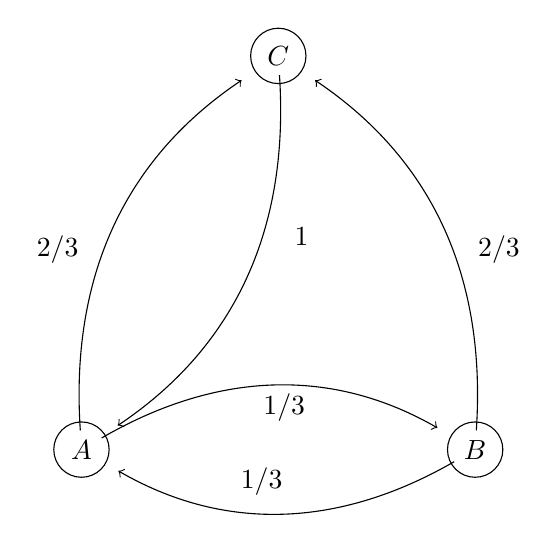
\begin{tikzpicture}
                        \node (A) at (0, 0) {$A$};
                        \node (B) at (5, 0) {$B$};
                        \node (C) at (2.5, 5) {$C$};

                        \draw (A) circle (10pt);
                        \draw (B) circle (10pt);
                        \draw (C) circle (10pt);

                        \draw[->, shorten >= 7pt] (A) to [bend left] (B) node[xshift=-0.85in, yshift=0.15in]{$1/3$};
                        \draw[->, shorten >= 7pt] (A) to [bend left] (C) node[xshift=-1in, yshift=-0.9in]{$2/3$};

                        \draw[->, shorten >= 7pt] (B) to [bend left] (A) node[xshift=0.8in, yshift=-0.1in]{$1/3$};
                        \draw[->, shorten >= 7pt] (B) to [bend right] (C) node[xshift=1in, yshift=-0.9in]{$2/3$};

                        \draw[->, shorten >= 7pt] (C) to [bend left] (A) node[xshift=1in, yshift=1in]{$1$};
                    \end{tikzpicture}
                \end{center}
                Notice that there is a path from every node to every other node (A and B are trivial and $C \to A \to B$). Thus, by theorem 1.3, $P$ is irreducible. $\qed$
            \color{black}

        \item (1 point) Prove that the Markov chain $\{X_n\}_{n=0}^\infty$ is aperiodic.
       
            \color{blue}
                The period of a Markov chain is given by $d = \gcd(I_i)$ where $I_i = \{n \geq 1\; | \; (P^n)_{ii} > 0\}$. 

                We calculate the first few powers:
                \begin{align*}
                    P^2 &= \begin{pmatrix}
                        7/9 & 0 & 2/9\\
                        6/9 & 1/9 & 2/9\\
                        0 & 3/9 & 6/9
                    \end{pmatrix}\\
                    P^3 &= \begin{pmatrix}
                        2/9 & 7/27 & 14/27\\
                        7/27 & 2/9 & 14/27\\
                        7/9 & 0 & 2/9
                    \end{pmatrix}\\
                \end{align*}

                And see that both $2\in I_i$ and $3 \in I_i$ for $i= \{1, 2, 3\}$ because both main diagonals are positive. But $2$ and $3$ are already coprime so no matter what other values are in $I_i$, the GCD is $1$ and the MC is aperiodic. $\qed$
            \color{black}
                
        \item (1 point) Compute the stationary distribution of the Markov chain $\{X_n\}_{n=0}^\infty$.
        
            \color{blue}
                By Theorem 1.2, as the MC is irreducible, its unique stationary distribution is given by $\vec \pi^T = \vec \pi^T P$
                
                \begin{align*}
                    \begin{pmatrix}
                        \pi(x_1) & \pi(x_2) & \pi(x_3)
                    \end{pmatrix} &= \begin{pmatrix}
                        \pi(x_1) & \pi(x_2) & \pi(x_3)
                    \end{pmatrix}\begin{pmatrix}
                        0 & 1/3 & 2/3\\
                        1/3 & 0 & 2/3\\
                        1 & 0 & 0
                    \end{pmatrix}\\
                    &= \begin{pmatrix}
                        \frac{1}{3}\pi(x_1) + \pi(x_3) & \frac{1}{3}\pi(x_1) & \frac{2}{3}\pi(x_1) + \frac{2}{3}\pi(x_2)
                    \end{pmatrix}
                \end{align*}
                Which gives a system we can put in terms of $\pi(x_1)$:
                \[\begin{cases}
                    \pi(x_1) = \frac{1}{3}\pi(x_1) + \pi(x_3)\\
                    \pi(x_2) = \frac{1}{3}\pi(x_1)\\
                    \pi(x_3) = \frac{2}{3}\pi(x_1) + \frac{2}{3}\pi(x_2)
                \end{cases} = \begin{cases}
                    \pi(x_1) = \pi(x_1)\\
                    \pi(x_2) = \frac{1}{3}\pi(x_1)\\
                    \pi(x_3) = \frac{2}{3}\pi(x_1) + \frac{2}{9}\pi(x_1) = \frac{8}{9}\pi(x_1)
                \end{cases}\]
               
                Further, we have that 
                \[\pi(x_1) + \pi(x_2) + \pi(x_3) = 1\]
                so 
                \[\pi(x_1) + \frac{1}{3}\pi(x_1) + \frac{8}{9}\pi(x_1) = \frac{20}{9}\pi(x_1) = 1 \implies \pi(x_1) = \frac{9}{20} \]
                
                Substituting back in, 
                \[\begin{cases}
                    \pi(x_1) = \frac{9}{20}\\
                    \pi(x_2) = \frac{1}{3}\cdot \frac{9}{20} = \frac{3}{20}\\
                    \pi(x_3) = \frac{8}{9}\cdot \frac{9}{20} = \frac{8}{20}
                \end{cases}\]
                so 
                \[\boxed{\vec \pi^T = \begin{pmatrix}
                    9/20\\
                    3/20\\
                    2/5
                \end{pmatrix}}\]
            \color{black}   
        
        \item (1 point) Suppose the function $f:\mathcal{X}\rightarrow\mathbb{R}$ is defined as follows
        \begin{align*}
            f(x_k)=k^2,\ \ \mbox{ for all }k=1,2,3.
        \end{align*}
        Compute the following value.
        \begin{align*}
            \sum_{x\in\mathcal{X}}f(x)\cdot\pi(x),
        \end{align*}
        where $\pi$ is the stationary distribution you derived in part (c).
        
            \color{blue}
                \begin{align*}
                    \sum_{x\in \mfX} f(x) \cdot \pi(x) &= f(x_1) \cdot \pi(x_1) + f(x_2) \cdot \pi(x_2) + f(x_3) \cdot \pi(x_3)\\
                        &= 1 \cdot \frac{9}{20} + 4\cdot \frac{3}{20} + 9\cdot \frac{2}{5}\\
                        &= \frac{9 + 12 + 72}{20}\\
                        &= \boxed{\frac{93}{20}}
                \end{align*}
            \color{black}

        \item (1 point) Compute the following limit
        \begin{align*}
            \lim_{n\rightarrow\infty} \boldsymbol{P}^n.
        \end{align*}
        (Hint: the limit is a 3-by-3 matrix.)

            \color{blue}
                Since the MC is irreducible and aperiodic, we can apply Theorem 1.4:

                \begin{align*}
                    \lim_{n \to \infty} P^n &= \begin{pmatrix}
                        \pi(x_1) & \pi(x_2) & \pi(x_3)\\
                        \pi(x_1) & \pi(x_2) & \pi(x_3)\\
                        \pi(x_1) & \pi(x_2) & \pi(x_3)
                    \end{pmatrix}\\
                    &= \boxed{\begin{pmatrix}
                        9/20 & 3/20 & 2/5\\
                        9/20 & 3/20 & 2/5\\
                        9/20 & 3/20 & 2/5
                    \end{pmatrix}}
                \end{align*}

            \color{black}

    \end{enumerate}
\end{enumerate}
%\bibliographystyle{plain}
\bibliography{sample}

\end{document}
